\documentclass[11pt,a4paper]{article}

\usepackage[margin=2.2cm]{geometry}
\usepackage{booktabs}
\usepackage{graphicx}
\usepackage{xcolor}
\usepackage{tabularx}
\usepackage{longtable}
\usepackage{enumitem}
\usepackage{xurl}        % allow line breaks inside long URLs
\usepackage[hidelinks]{hyperref}

\newcolumntype{Y}{>{\raggedright\arraybackslash}X}

\setlength{\emergencystretch}{3em}
\setlength{\parskip}{0.45em}
\setlength{\parindent}{0pt}

\title{\textbf{RAG: Baseline Retrieval vs.\ Cross-Encoder Re-Ranking}}
\author{Deepti Koranga}
\date{\today}

\begin{document}
\maketitle

\section*{Setup}
\begin{center}\begin{tabular}{ll}\toprule
\textbf{Item} & \textbf{Value} \\ \midrule
Document & D\&D Basic Rules (2018), Wizards of the Coast \\
Pages / chunks & 180 pages $\rightarrow$ 1119 chunks \\
Chunking & 774 chars mean, 150 overlap, page-bounded \\
Bi-encoder & \texttt{sentence-transformers/all-MiniLM-L6-v2} \\
Cross-encoder & \texttt{cross-encoder/ms-marco-MiniLM-L-6-v2} \\
Generator & \texttt{gemini-3-flash-preview}, temperature 0 \\
Retrieve / context & top 10 candidates, top 3 to the LLM \\
Stress queries & 15 \\
\bottomrule\end{tabular}\end{center}

Code and the executed notebook:
\url{https://github.com/DeeptiKoranga/rag-baseline-vs-reranking}

\section{Architecture Comparison}

Measured quantities relevant to this section:

\begin{center}\begin{tabular}{lr}\toprule
\textbf{Quantity} & \textbf{Measured} \\ \midrule
Chunk vectors embedded once, reused every query & $1119 \times 384$ \\
Query embedding (one forward pass) & 11.01 ms \\
Vector search over the whole corpus & 0.07 ms \\
Cross-encoder, 10 pairs & 57.30 ms \\
Cross-encoder, per (query, chunk) pair & 5.7 ms \\
\bottomrule\end{tabular}\end{center}
The two retrievers differ in \emph{when} the query and the chunk are allowed to
see each other. The bi-encoder embeds them separately: a chunk becomes a
384-dimensional vector that depends on nothing but the chunk, and the query
becomes a second vector that depends on nothing but the query. The only
interaction between them is the final cosine --- a single scalar collapsed out
of two independently formed summaries. The cross-encoder never forms those
summaries. It concatenates query and chunk into one sequence and runs full
self-attention over it, so every query token can attend to every chunk token,
and it emits one relevance score for that pair directly. Nothing resembling a
reusable chunk representation exists anywhere in that computation.

That difference is exactly what the timings above measure. Because the
bi-encoder's chunk vectors are query-independent, all $1119 \times 384$ of them
were embedded once at index time and are reused unchanged by every query since.
At query time only one forward pass remains --- 11.01~ms for the query
embedding --- and comparing it against the whole corpus is a single matrix
product, 0.07~ms, which is under one percent of the query-encoding cost. The
corpus is, in effect, free to search; what costs is encoding the query, and the
corpus size barely enters.

The cross-encoder has no such pre-computable half. Its score exists only for a
specific (query, chunk) pair, so it cannot be computed before the query arrives
and cannot be cached for the next one. All 10 pairs are joint forward passes
done fresh, 57.30~ms in total, 5.7~ms each, and that per-pair figure is the
whole story of the method: cost is linear in the number of pairs scored, with no
index, no reuse, and no amortisation available.

So the two models are not competing implementations of the same idea; they
occupy opposite ends of a precision/pre-computation trade. The bi-encoder buys
corpus-scale search by giving up query--chunk interaction, which is why it is
the only thing that can look at 1119 chunks at all. The cross-encoder buys
query--chunk interaction by giving up pre-computation, which is why it can only
ever be shown a shortlist. The two-stage pipeline is the direct consequence:
one model to make a candidate set cheaply, the other to order it well, with the
candidate size chosen as a budget for the second model rather than a property of
the corpus.

\section{Qualitative and Rank Shift Analysis}

\subsection{How a failure is measured}

For each query the chunk that actually answers it is pinned in advance by a
regular expression matching a phrase unique to that chunk. Every claim below
is therefore a rank, not an impression. \textit{rank$_{100}$} is the
answer-bearing chunk's position in a top-100 bi-encoder sweep (diagnostic
only); \textit{base} and \textit{rerank} are its position among the 10
candidates before and after the cross-encoder. A dash means absent from that
set. A query is \textbf{rescued} when the answer chunk was outside the top 3
for the baseline and inside it after re-ranking.

\subsection{Full rank table}
\begin{center}\footnotesize\begin{tabular}{llrrrrcl}\toprule
\textbf{ID} & \textbf{Category} & \textbf{p.} & \textbf{rank$_{100}$} & \textbf{base} & \textbf{rerank} & \textbf{shift} & \textbf{Outcome} \\ \midrule
Q1 & Keyword trap/distractor & 46 & 6 & 6 & 7 & $-1$ & still missed \\
Q2 & Keyword trap/distractor & 54 & 2 & 2 & 1 & $+1$ & already in top 3 \\
Q3 & Keyword trap/distractor & 63 & 1 & 1 & 2 & $-1$ & already in top 3 \\
Q4 & Exception/corner case & 166 & 98 & -- & -- & -- & beyond recall \\
Q5 & Exception/corner case & 70 & 2 & 2 & 2 & 0 & already in top 3 \\
Q6 & Exception/corner case & 46 & 3 & 3 & 1 & $+2$ & already in top 3 \\
Q7 & Negation/constraint & 77 & 2 & 2 & 1 & $+1$ & already in top 3 \\
Q8 & Negation/constraint & 84 & -- & -- & -- & -- & beyond recall \\
Q9 & Negation/constraint & 72 & 5 & 5 & 1 & $+4$ & \textbf{rescued} \\
Q10 & Buried vital chunk & 68 & 1 & 1 & 1 & 0 & already in top 3 \\
Q11 & Buried vital chunk & 67 & 6 & 6 & 1 & $+5$ & \textbf{rescued} \\
Q12 & Buried vital chunk & 67 & 2 & 2 & 2 & 0 & already in top 3 \\
Q13 & Buried vital chunk & 68 & 5 & 5 & 8 & $-3$ & still missed \\
Q14 & Keyword trap/distractor & 77 & 5 & 5 & 1 & $+4$ & \textbf{rescued} \\
Q15 & Control & 79 & 1 & 1 & 1 & 0 & already in top 3 \\
\bottomrule\end{tabular}\end{center}
\begin{center}\begin{tabular}{lr}\toprule
\textbf{Summary} & \textbf{Count} \\ \midrule
Queries & 15 \\
Answer chunk in top 3 -- baseline & 8 \\
Answer chunk in top 3 -- re-ranked & 11 \\
Rescued by re-ranking & 3 \\
Never retrieved (re-ranking cannot help) & 2 \\
Retrieved but still outside top 3 & 2 \\
\bottomrule\end{tabular}\end{center}
\subsection{Rank shifts, with what the baseline ranked instead}
\subsubsection*{Q9 --- Negation / constraint --- Rank \#5 $\rightarrow$ Rank \#1}
\textbf{Query:} \textit{When am I prohibited from acting at all at the start of a battle?}

\textbf{Why it is hard:} Negative phrasing against a chapter full of 'you can' statements.

\textbf{Baseline top 3 (cosine)}
\begin{center}\footnotesize\begin{tabularx}{\textwidth}{rrrrcY}\toprule
\textbf{\#} & \textbf{was} & \textbf{p.} & \textbf{chunk} & \textbf{cosine} & \textbf{text} \\ \midrule
1 & -- & 72 & 509 & 0.419 & nonplayer characters involved in combat, and each other pl  \\
2 & -- & 72 & 508 & 0.367 & The clatter of a sword striking against a shield. The terr  \\
3 & -- & 162 & 1031 & 0.365 & until the start of its next turn. Actions Greataxe. Melee   \\
\bottomrule\end{tabularx}\end{center}
\textbf{Re-ranked top 3 (cross-encoder)}
\begin{center}\footnotesize\begin{tabularx}{\textwidth}{rrrrcY}\toprule
\textbf{\#} & \textbf{was} & \textbf{p.} & \textbf{chunk} & \textbf{score} & \textbf{text} \\ \midrule
1 & \#5 & 72 & 511 & -7.001 & If you're surprised, you can't move or take an action on y \textbf{$\leftarrow$ ANSWER} \\
2 & \#3 & 162 & 1031 & -8.203 & until the start of its next turn. Actions Greataxe. Melee   \\
3 & \#9 & 73 & 517 & -9.533 & The DM might require you to use an action for any of these  \\
\bottomrule\end{tabularx}\end{center}

\subsubsection*{Q11 --- Buried vital chunk --- Rank \#6 $\rightarrow$ Rank \#1}
\textbf{Query:} \textit{Does scrambling up a wall or wading through a swamp slow me down?}

\textbf{Why it is hard:} The movement-cost rule is phrased in feet, not in 'slow down'.

\textbf{Baseline top 3 (cosine)}
\begin{center}\footnotesize\begin{tabularx}{\textwidth}{rrrrcY}\toprule
\textbf{\#} & \textbf{was} & \textbf{p.} & \textbf{chunk} & \textbf{cosine} & \textbf{text} \\ \midrule
1 & -- & 66 & 459 & 0.395 & Movement Swimming across a rushing river, sneaking down a   \\
2 & -- & 73 & 520 & 0.384 & If you have more than one speed, such as your walking spee  \\
3 & -- & 73 & 522 & 0.377 & A. You can drop prone without using any of your speed. Sta  \\
\bottomrule\end{tabularx}\end{center}
\textbf{Re-ranked top 3 (cross-encoder)}
\begin{center}\footnotesize\begin{tabularx}{\textwidth}{rrrrcY}\toprule
\textbf{\#} & \textbf{was} & \textbf{p.} & \textbf{chunk} & \textbf{score} & \textbf{text} \\ \midrule
1 & \#6 & 67 & 468 & -8.171 & Difficult Terrain The travel speeds given in the Travel Pa \textbf{$\leftarrow$ ANSWER} \\
2 & \#1 & 66 & 459 & -8.270 & Movement Swimming across a rushing river, sneaking down a   \\
3 & \#5 & 73 & 521 & -8.879 & treacherous staircases---the setting of a typical fight cont  \\
\bottomrule\end{tabularx}\end{center}

\subsubsection*{Q14 --- Keyword trap / distractor --- Rank \#5 $\rightarrow$ Rank \#1}
\textbf{Query:} \textit{Can I attack with a weapon in each hand on the same turn?}

\textbf{Why it is hard:} The Fighter class has a feature \textit{called} 'Two-Weapon Fighting', which is not the rule -- the rule, with its 'light' restriction, is 50 pages later in the combat chapter.

\textbf{Baseline top 3 (cosine)}
\begin{center}\footnotesize\begin{tabularx}{\textwidth}{rrrrcY}\toprule
\textbf{\#} & \textbf{was} & \textbf{p.} & \textbf{chunk} & \textbf{cosine} & \textbf{text} \\ \midrule
1 & -- & 27 & 193 & 0.403 & Two-Weapon Fighting When you engage in two-weapon fighting  \\
2 & -- & 77 & 550 & 0.389 & unless that modifier is negative. If either weapon has the  \\
3 & -- & 27 & 197 & 0.381 & or (b) two handaxes $\bullet$ (a) a dungeoneer's pack or (b) an ex  \\
\bottomrule\end{tabularx}\end{center}
\textbf{Re-ranked top 3 (cross-encoder)}
\begin{center}\footnotesize\begin{tabularx}{\textwidth}{rrrrcY}\toprule
\textbf{\#} & \textbf{was} & \textbf{p.} & \textbf{chunk} & \textbf{score} & \textbf{text} \\ \midrule
1 & \#5 & 77 & 549 & 2.119 & modifier---the same modifier used for the attack roll---to the \textbf{$\leftarrow$ ANSWER} \\
2 & \#1 & 27 & 193 & 1.577 & Two-Weapon Fighting When you engage in two-weapon fighting  \\
3 & \#7 & 73 & 516 & 1.445 & Other Activity on Your Turn Your turn can include a variet  \\
\bottomrule\end{tabularx}\end{center}

\subsection{Cases where re-ranking did not help}
\begin{itemize}[leftmargin=1.2em,itemsep=3pt]
\item \textbf{Q4} (Exception / corner case) --- \textit{beyond recall.} The answer chunk on p.~166 sits at rank 98 of a top-100 sweep, so it never enters the 10 candidates and no re-ranker can reach it. Query: \textit{If a fight comes at us in several waves, can we rest in between to heal up?}
\item \textbf{Q8} (Negation / constraint) --- \textit{beyond recall.} The answer chunk on p.~84 does not appear in a top-100 sweep at all, so it never enters the 10 candidates and no re-ranker can reach it. Query: \textit{What will make me lose a spell I am trying to keep going?}
\item \textbf{Q1} (Keyword trap / distractor) --- \textit{still missed.} Retrieved at \#6, re-ranked to \#7, still outside the top 3. Query: \textit{Does wearing heavy plate make it harder to sneak past guards unnoticed?}
\item \textbf{Q13} (Buried vital chunk) --- \textit{still missed.} Retrieved at \#5, re-ranked to \#8, still outside the top 3. Query: \textit{How much damage do you take from a long drop?}
\end{itemize}
\subsection{Answer 1 vs.\ Answer 2}
\subsubsection*{Q14 --- Can I attack with a weapon in each hand on the same turn?}
\textbf{Answer 1 (baseline)} --- context pages [27, 77, 27], chunks [193, 550, 197]:
\begin{quote}\itshape Based on the provided context, you can engage in two-weapon fighting. When doing so, you can add your ability modifier to the damage of the second attack, unless that modifier is negative (p. 27, 77). If either weapon has the thrown property, you may throw it instead of making a melee attack (p. 77). Additionally, if you are at least 2nd level, you can use Action Surge to take one additional action on your turn, which increases to two uses at 17th level (p. 27). You must finish a short or long rest before using Action Surge again (p. 27).\end{quote}
\textbf{Answer 2 (re-ranked)} --- context pages [77, 27, 73], chunks [549, 193, 516]:
\begin{quote}\itshape Yes, when you take the Attack action with a light melee weapon in one hand, you can use a bonus action to attack with a different light melee weapon in the other hand (p. 77). If either weapon has the thrown property, you may throw it instead of making a melee attack (p. 77). Restrictions and penalties include: * Both weapons must be light melee weapons (p. 77). * You do not add your ability modifier to the damage of the bonus attack unless the modifier is negative (p. 77). However, certain class features allow you to add the modifier to the second attack's damage (p. 27).\end{quote}

\subsubsection*{Q9 --- When am I prohibited from acting at all at the start of a battle?}
\textbf{Answer 1 (baseline)} --- context pages [72, 72, 162], chunks [509, 508, 1031]:
\begin{quote}\itshape NOT IN CONTEXT.\end{quote}
\textbf{Answer 2 (re-ranked)} --- context pages [72, 162, 73], chunks [511, 1031, 517]:
\begin{quote}\itshape You are prohibited from moving or taking an action on your first turn of combat if you are surprised (p. 72). Additionally, you are restricted from taking any reactions until that first turn ends (p. 72). While a reaction is an instant response to a trigger that can occur on your turn or someone else's, once you use a reaction, you are prohibited from taking another one until the start of your next turn (p. 73).\end{quote}

\subsubsection*{Q11 --- Does scrambling up a wall or wading through a swamp slow me down?}
\textbf{Answer 1 (baseline)} --- context pages [66, 73, 73], chunks [459, 520, 522]:
\begin{quote}\itshape Yes. According to the rules for difficult terrain, every foot of movement costs 1 extra foot (p. 73). The context identifies boulder-strewn caverns, briar-choked forests, and treacherous staircases as examples of settings containing difficult terrain (p. 73). Additionally, scaling a treacherous mountain slope or swimming across a rushing river are noted as key types of movement in adventures (p. 66). While the DM may summarize movement between encounters without calculating exact distances, it is sometimes important to determine how long it takes to travel between spots in days, hours, or minutes (p. 66).\end{quote}
\textbf{Answer 2 (re-ranked)} --- context pages [67, 66, 73], chunks [468, 459, 521]:
\begin{quote}\itshape Yes. Climbing and swimming (such as wading through a swamp) are special types of movement where each foot costs 1 extra foot of speed (p. 67). If the terrain is considered difficult terrain---such as deep swamps, steep mountains, or rubble---you move at half speed, meaning 1 foot of movement costs 2 feet of speed (p. 67). When climbing or swimming in difficult terrain, each foot costs 2 extra feet (p. 67). Additionally, the travel speeds for simple terrain assume you can cover only half the normal distance in a minute, hour, or day when in difficult terrain (p. 67). This rule applies even if multiple factors in a space count as difficult terrain (p. 73).\end{quote}

\subsubsection*{What the three rescues actually fixed}

The three rescued queries move the answer chunk from \#5, \#6 and \#5 to \#1,
but they were failing in two quite different ways, and only one of them is the
failure people usually picture.

\textbf{Q9 and Q11 are retrieval failures that the generator declined to
paper over.} For Q9 the baseline's three chunks were a definition of ``you''
(p.~72), the chapter's scene-setting opening paragraph (p.~72) and a greataxe
stat block (p.~162) --- cosine 0.419, 0.367, 0.365, a flat and uninformative
spread. Nothing in that context contains the surprise rule, and the generator
said so: \textit{NOT IN CONTEXT}. That is the best possible behaviour from a
model handed the wrong evidence, and it means the baseline's failure here is
entirely a retrieval failure; the generation stage was never the problem. After
re-ranking, chunk 511 --- \textit{``If you're surprised, you can't move or take
an action\ldots''} --- is \#1, and Answer 2 states the rule with both of its
clauses, the action ban and the reaction ban. Note that the cross-encoder
reaches this while scoring it $-7.0$: the absolute scores for Q9 are all
strongly negative, so what re-ranking supplies is a usable \emph{ordering},
not calibrated confidence.

Q11 is the softer version of the same shape. The baseline did not refuse ---
it answered ``Yes'' and even quoted the difficult-terrain cost correctly --- but
it got there from chunk 522, which mentions difficult terrain in passing, and
it padded the rest of the answer with travel-time bookkeeping from p.~66 that
the question did not ask about. The specific thing asked --- whether
\emph{climbing} and \emph{swimming} cost extra --- is in chunk 468, which the
baseline ranked \#6 and never showed the LLM. So Answer 1 is not false; it is
answering a neighbouring question. Answer 2, with chunk 468 at \#1, separates
the two mechanisms the question conflates: climbing and swimming cost 1 extra
foot per foot, difficult terrain costs 1 extra foot, and the two stack to 2
extra feet when combined. That distinction is the actual answer, and it is
invisible in Answer 1.

\textbf{Q14 is the dangerous one: the baseline answered confidently and was
wrong.} The query asks whether you can attack with a weapon in each hand. The
bi-encoder's top hit, at the highest cosine in the set (0.403), is the Fighter
class feature \emph{named} ``Two-Weapon Fighting'' on p.~27 --- a feature that
modifies the rule but is not the rule. The actual rule, 50 pages later, carries
the restriction that both weapons must be \emph{light} and that the second
attack uses a bonus action. Given the class feature instead, the generator
produced a fluent answer that states you may add your ability modifier to the
second attack's damage --- which is the \emph{exception} granted to Fighters,
presented as the general rule --- and then drifted into Action Surge, which has
nothing to do with the question. There is no hedge and no refusal. A reader
with no Fighter levels would take away a rule that does not apply to them, and
nothing in Answer 1 would warn them. Answer 2, built on chunk 549 at \#1,
leads with the bonus-action mechanic, states the \emph{light} restriction
explicitly, states that the modifier is \emph{not} added by default, and then
correctly demotes the Fighter feature to the exception it is.

Those are the two failure shapes worth distinguishing. Q9 and Q11 degrade
\emph{visibly} --- a refusal, or an answer that is obviously about something
adjacent --- and a user can tell something went wrong. Q14 degrades
\emph{invisibly}: same confident register, same page citations, substantively
wrong content. Keyword-trap queries are precisely the ones that produce the
second shape, because the distractor that wins on cosine is topically correct
and merely not authoritative, so the generator has every reason to sound sure.
The cross-encoder helps here for a structural reason: scoring the pair jointly
lets it register that the p.~27 chunk is \emph{about} two-weapon fighting
without \emph{answering} whether you may do it, a distinction a cosine between
two independent summaries cannot express.

\subsubsection*{What re-ranking did not fix, and why}

The four remaining failures split cleanly into two groups, and the split
matters more than the count.

\textbf{Q4 and Q8 are beyond recall, and this is a ceiling, not a tuning
problem.} Q8's answer chunk on p.~84 does not appear in a top-100 bi-encoder
sweep at all; Q4's sits at rank 98, nine times deeper than the candidate
window. A re-ranker can only reorder what it is given, so for these two it was
never in the game --- the pipeline's recall ceiling is fixed entirely by stage
one, and no amount of cross-encoder quality raises it. Both are also
vocabulary mismatches rather than ranking mistakes: Q8 asks what makes you
``lose a spell I am trying to keep going'' against a rulebook that says
``concentration''; Q4 asks about resting between waves of a fight against text
organised under short and long rests. The bi-encoder is being asked to bridge a
gap it has no mechanism for. The fixes are all at stage one --- a larger
candidate window, hybrid lexical scoring, or query expansion --- not at stage
two.

\textbf{Q1 and Q13 are the honest cost of re-ranking.} Both were retrieved
inside the candidate set and both were pushed \emph{further away} by the
cross-encoder: Q1 from \#6 to \#7, Q13 from \#5 to \#8. The cross-encoder is a
model, not an oracle, and on these two its judgement was worse than cosine's.
Q13 in particular moves three places in the wrong direction. It is worth being
precise about the damage, though: neither query was in the top 3 before
re-ranking either, so in both cases the LLM saw a wrong context under both
pipelines and the regression changed nothing the user could observe. Across all
15 queries no answer chunk was dropped \emph{out} of the top 3 by re-ranking;
the only regression that touched a top-3 chunk was Q3's \#1 to \#2, which stays
inside the context window. So on this set the cross-encoder's errors were
confined to candidates that were already lost.

\subsubsection*{Net effect}

Answer-chunk presence in the top 3 goes from 8/15 to 11/15 --- the three
rescues, with no losses. Two of the four remaining failures are structurally
out of the re-ranker's reach, which means that of the four queries where
re-ranking \emph{could} have helped, it helped on three. The one real
disappointment is Q13. That is a meaningful gain on a deliberately adversarial
set, and it is worth remembering that the set is adversarial: the control
query, Q15, was already \#1 and stayed \#1, which is what the whole easy
majority of real traffic looks like. Re-ranking earns its cost on the hard tail,
not on the median query.

\section{Latency Profiling}

15 queries $\times$ 5 repeats $=$ 75 measurements per pipeline, after one
untimed warm-up pass. The LLM call is excluded from the pipeline comparison:
it is identical work in both pipelines and its variance is far larger than
the retrieval times under test. It is reported separately below.

\begin{center}\begin{tabular}{lrrrrr}\toprule
\textbf{Stage} & \textbf{mean} & \textbf{median} & \textbf{p95} & \textbf{min} & \textbf{max} \\
 & (ms) & (ms) & (ms) & (ms) & (ms) \\ \midrule
Query embedding (1 pass) & 11.01 & 11.18 & 12.21 & 6.84 & 13.71 \\
Vector search (whole corpus) & 0.07 & 0.06 & 0.07 & 0.05 & 0.37 \\
Cross-encoder (10 pairs) & 57.3 & 48.34 & 110.96 & 37.45 & 114.11 \\
\midrule
\textbf{Pipeline 1 retrieval} & \textbf{11.08} & 11.24 & 12.32 & 6.9 & 13.77 \\
\textbf{Pipeline 2 retrieval} & \textbf{68.38} & 59.99 & 121.62 & 44.87 & 125.68 \\
\bottomrule\end{tabular}\end{center}

Pipeline 2 retrieval costs $\mathbf{6.2\times}$ Pipeline 1
($\mathbf{+57}$ ms absolute). Measured separately, the LLM call averages
$\mathbf{34674}$ ms over 6 calls, so against generation the re-ranker adds
$\mathbf{0.2\%}$ to end-to-end latency --- the generator dominates by
roughly $605\times$.


\begin{figure}[h]\centering
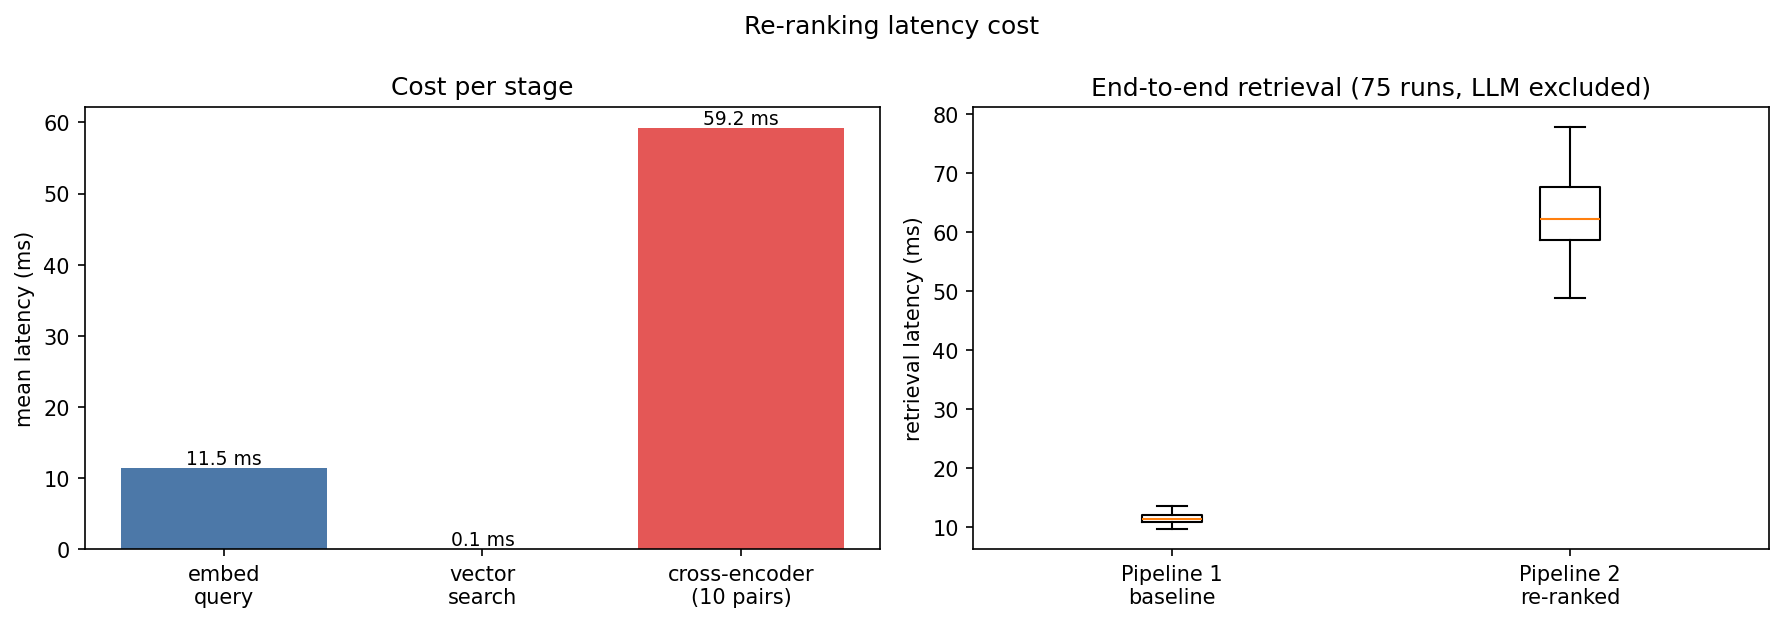
\includegraphics[width=\textwidth]{../figures/latency.png}
\caption{Per-stage cost (left) and end-to-end retrieval latency (right).}
\end{figure}

Within retrieval, the cost structure is stark and entirely one-sided. Vector
search over the full corpus is 0.07~ms --- genuinely negligible, 0.6\% of the
query embedding it follows. Pipeline 1 is therefore not really ``embed and
search''; it is ``embed'', with a rounding error attached. The entire 57~ms
difference between the pipelines is the cross-encoder, and that is the only
line in the table that grows with the candidate count.

The cross-encoder is also the only stage with an unpleasant distribution. Its
p95 of 110.96~ms is 2.3$\times$ its median of 48.34~ms, and min-to-max spans
37.45--114.11~ms --- a 3$\times$ spread for what is nominally the same work on
the same 10 pairs. Query embedding, by contrast, is tight: median 11.18~ms,
p95 12.21~ms. The variance is almost certainly chunk length --- a joint forward
pass is quadratic in sequence length, and candidate chunks vary in size --- so
the re-ranker's cost is governed by the \emph{content} of the shortlist, not
just its length. At the tail this matters more than the mean suggests: Pipeline
2's p95 is 121.62~ms against Pipeline 1's 12.32~ms, a 9.9$\times$ ratio, worse
than the 6.2$\times$ at the mean. Any latency budget written against the mean
will be wrong in the direction that hurts.

So there are two defensible framings of the same number, and they genuinely
disagree. Measured against retrieval, re-ranking is a 6.2$\times$ tax. Measured
against the end-to-end request, the generator's 34{,}674~ms mean swamps
everything: 57~ms is 0.2\% of the user's wait, and the LLM outweighs the
re-ranker by roughly 605$\times$. On the figures as collected, the second
framing is the one to design against. A user waiting roughly 35 seconds for an
answer cannot perceive 57~ms, and spending 0.2\% of the latency budget to move
answer-chunk presence from 8/15 to 11/15 is not a close call --- it is the
cheapest quality improvement available anywhere in this system. Optimising the
6.2$\times$ would be optimising the component that is already 0.2\% of the
total.

Two caveats keep that from being unconditional. First, the comparison is
unfair to the re-ranker's critics in a specific way: 34.7~s is a hosted-API
call over the network, measured over only 6 calls, and it is dominated by
network and queueing rather than computation. Against a fast local generator,
or a streaming setup judged on time-to-first-token rather than
time-to-completion, the denominator shrinks and 57~ms stops being invisible.
Second, the argument is about \emph{latency}, not throughput. Per-request the
re-ranker is free; per-server it is 57~ms of occupied compute per query, which
is a capacity cost that does not disappear just because the user cannot feel
it. The right reading is that re-ranking should be defaulted on for any
pipeline that ends in a generator call, and reconsidered only where retrieval
is the product --- a search box returning links, an autocomplete, a
retrieval-only API --- because there the 6.2$\times$ is the whole user-visible
latency and the trade reverses.

\section{Scaling: Why Not Cross-Encode Everything?}

The cross-encoder costs 5.7~ms per (query, chunk) pair and is linear in the
number of pairs, because a score exists only for a specific pair and nothing
can be precomputed between queries.

\begin{center}\begin{tabular}{lrrrr}\toprule
\textbf{Corpus} & \textbf{Chunks} & \textbf{Cross-encode all} & \textbf{Two-stage} & \textbf{Ratio} \\
 & & (s/query) & (s/query) & \\ \midrule
This rulebook & 1,119 & 6.4 & 0.068 & 94$\times$ \\
10k chunks & 10,000 & 57.3 & 0.068 & 838$\times$ \\
1M chunks & 1,000,000 & 5,730.0 & 0.068 & 83,796$\times$ \\
\bottomrule\end{tabular}\end{center}
The arithmetic settles the question on its own. Even on this small rulebook,
cross-encoding all 1119 chunks would take 6.4~s per query --- already longer
than most users will wait, and this is a 180-page PDF. At 10k chunks it is
57~s; at 1M it is 95 minutes for a single query. The two-stage column does not
move at all, because the shortlist stays at 10 pairs no matter how large the
corpus grows. That constant is the entire point: in a two-stage pipeline the
expensive model's cost is set by a budget you choose, while in the exhaustive
design it is set by a corpus size you do not control.

But the cost argument alone would only be an argument for a faster
cross-encoder, and that is why the structural argument matters more. The
bi-encoder's chunk vectors are query-independent: a chunk's embedding is a
function of the chunk alone, so it can be computed once at index time, stored,
and reused by every query forever --- which is exactly what the $1119 \times
384$ matrix in Section~1 is. Query-independence is also what makes an
\emph{index} possible. Because every chunk occupies a fixed point in a metric
space, that space can be partitioned, clustered or graph-linked in advance, and
a query can reach its neighbours while touching a small fraction of the corpus.
This is the mechanism behind every ANN index, and it is what lets vector search
cost 0.07~ms.

The cross-encoder forfeits all of that. A cross-encoder score is a function of
the pair, so it does not exist until the query arrives, there is nothing to
store at index time, and --- crucially --- the scores do not live in a metric
space at all. There is no chunk-side object to index, no triangle inequality to
prune with, no notion of two chunks being ``near'' each other independently of
the query. So sub-linear search is not merely unimplemented; it is structurally
unavailable. Every chunk must be scored because there is no cheap way to prove
in advance that any chunk can be skipped. Hardware changes the constant and
never the exponent: a cross-encoder 100$\times$ faster still takes 57~s per
query at 1M chunks, and still scales linearly while the corpus grows.

This is why the sensible architecture is not a choice between the two models
but a composition of them. The bi-encoder's cheapness buys \emph{coverage} ---
it is the only thing that can consider the whole corpus --- and the
cross-encoder's precision buys \emph{ordering} within whatever the first stage
hands it. Each supplies what the other structurally cannot.

The bill for that composition is in Section~2, and it should be stated plainly
rather than hidden in the ratio column. Q4 and Q8 fail because their answer
chunks never enter the top 10; Q8's does not appear in a top-100 sweep at all.
An exhaustive cross-encoder would very likely have found both --- it is the
precise model, and these are precisely the vocabulary-mismatch cases it handles
well. The two-stage design gave those two queries up in exchange for a 94$\times$
speedup on this corpus, and that trade is hard-coded: the pipeline's recall
ceiling is whatever stage one puts in the candidate set, and stage two can only
reorder beneath it. 13 of 15 answer chunks were reachable; 2 were not, and no
cross-encoder improvement will ever recover them.

That also says where the remaining engineering effort belongs. Having bought
coverage with the bi-encoder, the useful levers are all on stage one's recall,
not stage two's precision: widen the candidate window (at 5.7~ms per pair, going
from 10 to 50 candidates costs 228~ms --- still 0.7\% of the generator's
34.7~s, and it would have pulled Q4's rank-98 chunk no closer, but it buys
headroom cheaply), add lexical or hybrid scoring so that ``concentration''
can be reached from ``keep a spell going'', or expand queries before embedding
them. The re-ranker is already doing its job on three of the four queries it
could reach. The ceiling above it is the part that is not yet paid for.

\end{document}
